\documentclass[10pt]{article}
\usepackage[utf8]{inputenc}
\usepackage{amsmath}
\usepackage{amssymb}
\usepackage{graphicx}
\usepackage{hyperref}
\usepackage{menukeys}
\usepackage{nameref}
\usepackage{listings}
\usepackage{scrpage2}
\pagestyle{scrheadings}
\ifoot{\textsuperscript{\textcopyright} 2016-2020 Research group REMEX, Hochschule der Medien (Stuttgart, Germany) Licence: Apache 2.0 found \href{https://github.com/REMEXLabs/OpenAPE/blob/master/openAPE/license.txt}{here}.}
\title{OpenAPE}
\author{Stephan Unfried}
\date{\today} 
\begin{document}
\maketitle
\newpage
\tableofcontents
\newpage
\section{Introduction}
OpenAPE is a settings-based personalization framework to cover three important scenarios:

The bread and butter scenario is to **infer settings** for an application a user might not have met yet, for example using an Android phone for the first time with only using Windows PCs so far. In this use case, OpenAPE will try to find other users who have similar settings, but also have settings for the new target device or application. To do so, OpenAPE deploys various machine learning techniques, such as clustering existing users and creating virtual user profiles for these clusters. The fundamental assumption here is that users will adapt their device to their needs or preferences and thus settings applied by a users can be considered verified.

Quite similar to settings-adaptation scenario is **inferring content**. When coupled with a content server, OpenAPE can deliver content for webpages, such as images, that match a users settings, for example delivering a high-contrast image if respective settings are present for screen readers or magnifiers. There are, however, some subtle differences: it is hard to assess whether the content delivered was actually a good choice in the current situation. Further, content nowadays can range from simple images up to whole web apps, which in turn will invoke their own adaptation queries.

Finally, as a mix of the above use cases, OpenAPE could be used to **transfer rules and scripts to a user**, based on their preferences. Consider, for example, a smart home where the configuration for dimming lights in the evening or altering the lighting colour are complex, even time-dependent scripts. These scripts could be shipped to a user similar to simple content, but they have many configuration dimensions themselves, such as scaling with preferred light intensity etc.
\section{project structure}
\subsection{Modules}
The project consists of tree parts, represented in tree maven modules. For details of the associations see figure \ref{fig:moduleuml}.
\begin{figure}[b]
\centering
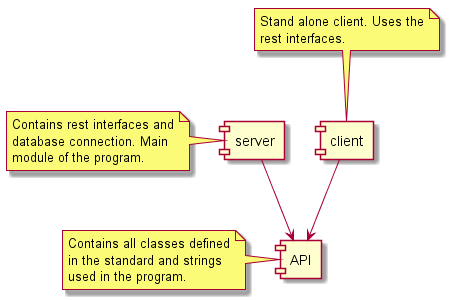
\includegraphics[width=0.8\textwidth]{uml/modulesuml.png}
\caption{module diagram.}
\label{fig:moduleuml}
\end{figure}
\subsection{API}
API contains classes and class structure used by the application server and clients who want to communicate with it. The classes contained in the API module represent the objects stored in the application. For clients it is important to uphold the class structure for the server to recognize those objects. For the structure of the module see figure \ref{fig:apiuml}.
\begin{figure}[b]
\centering
\makebox[\textwidth][c]{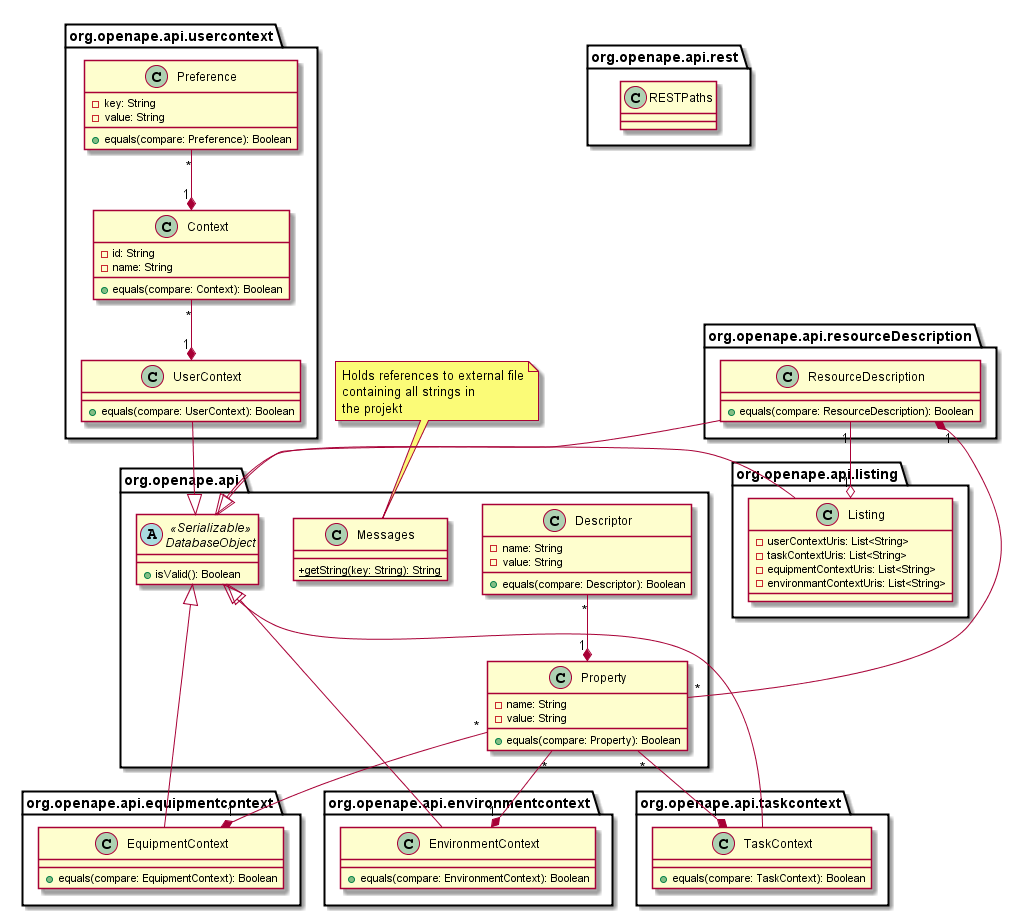
\includegraphics[width=1.4\textwidth]{uml/apiuml.png}}
\caption{API module structure diagram.}
\label{fig:apiuml}
\end{figure}
\subsection{Server}
\label{subsec:server}
The Server module is the main module of the application. It contains the web application used to up- and download contents. It provides an rest interface for access and uses a MongoDB and the file system to store data. The \emph{MongoDB} access can be configured in \directory{tomcat/webapps/<current application name on the server>/classes/config/mongo.properties}. For using the rest paths see the \emph{ISO-IEC\_CD\_24752-8} Standard. For the module structure see figure \ref{fig:serveruml}.
\begin{figure}[b]
\centering
\makebox[\textwidth][c]{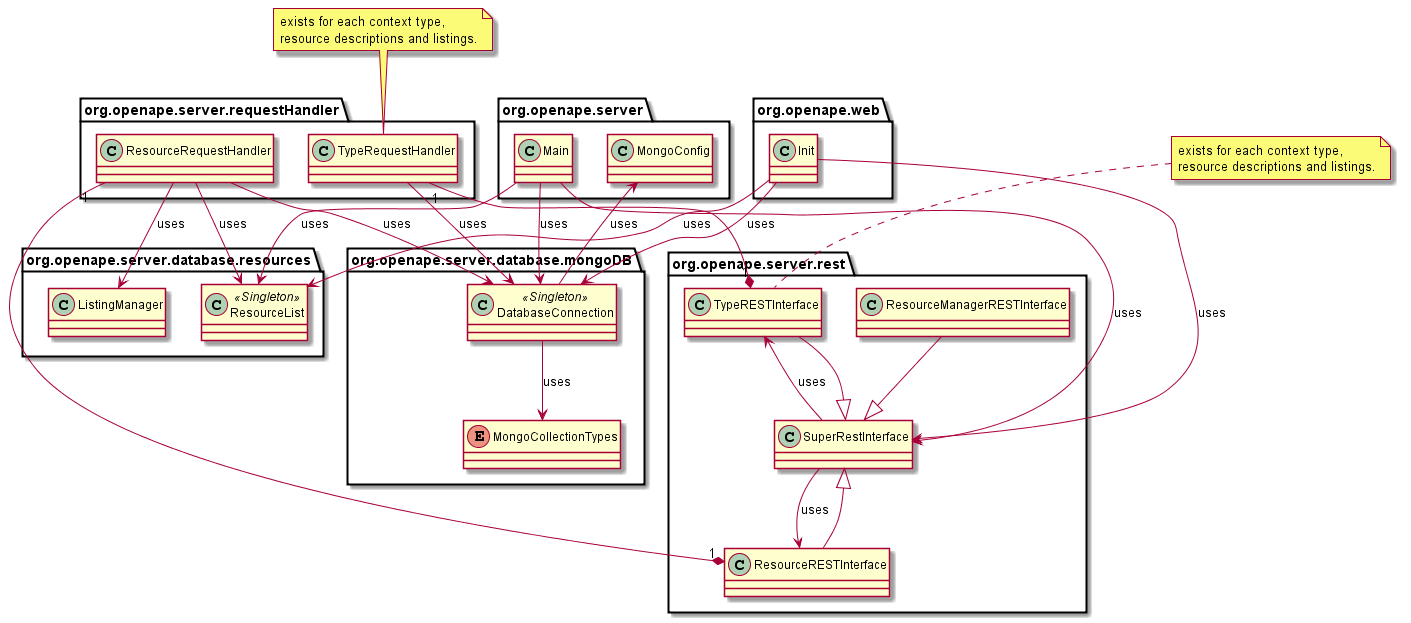
\includegraphics[width=1.6\textwidth]{uml/serveruml.png}}
\caption{Server module structure diagram.}
\label{fig:serveruml}
\end{figure}
\subsection{Client}
The Client is a sand alone module that uses the rest interface of the server to communicate with it. It can be replaced by any application capable of generating rest requests and processing the result.
\section{Get started with the project}
\paragraph{Remark} This section shows how to set up a development environment to work with the project. To see how to deploy the application for use please skip forward to section \nameref{sec:setupapp}.
\subsection{Git repository}
To use the repository used for this project you need a \emph{Github} account and an application capable of running git commands.
\subsubsection{Create Github account} To create an account visit \href{https://github.com/}{github.com}.
\subsubsection{Install Git application} On \emph{Linux} systems use your package installer to install a current git package. You can use the normal shell to run git commands. On \emph{Windows} you can use the \emph{Github} application from \href{https://github.com/}{github.com} and the build in git shell to run git commands.
\subsubsection{Clone Git repository} To clone the repository use your console, which is able to use git commands, and navigate to the location where it should be cloned to. Then use \texttt{git clone https://github.com/REMEXLabs/OpenAPE}. You will be asked so sign in with your \emph{Github} credentials.
\subsection{Eclipse}
The project is developed in \emph{Eclipse} and so here is described how to use it. But any IDE can be used that provides \emph{Maven} support.
\subsubsection{Install Eclipse} The current version of \emph{Eclipse} can be found on \href{https://eclipse.org/downloads/}{eclipse.org/downloads/}.
\subsubsection{Install Java} To develop this project with \emph{Eclipse} you need a current \emph{Java Development Kit}. Use the download button under \emph{JDK} \href{http://www.oracle.com/technetwork/java/javase/downloads/index.html}{oracle.com/technetwork/java/javase/downloads/index.html} to get the current version.
\subsubsection{Import project} It is recommended not to use the project folder as workspace for \emph{Eclipse} but to import the project. To do so start \emph{Eclipse} and navigate $File \rightarrow Import... \rightarrow Maven \rightarrow \text{\emph{Existing Maven Projects}} \rightarrow Next \rightarrow Browse... \rightarrow \text{browse the folder OpenAPE/openAPE} \rightarrow -> Finish$. Now you should have the main project plus the modules \emph{API} \emph{client} and \emph{server} in your navigation.
\subsubsection{Ensure the right Java version is used} The project will not work correctly if \emph{Eclipse} doesn't use the previously installed \emph{Java JDK} but a \emph{Java RE}. To change the used \emph{Java version} mark a module and navigate $Project \rightarrow Properties \rightarrow \text{emph{Java Build Path}} \rightarrow Libraries \rightarrow \text{mark the used system library} \rightarrow Edit... \rightarrow \text{emph{Execution environment}} \rightarrow \text{Choose a Java 1.8 JDK or newer from the list and klick finish. If none is available navigate \emph{Installed JREs…}} \rightarrow Search... \rightarrow  \text{Choose the installation path of the previously installed Java JDK. It should now be available in the execution environment list}.$ Repeat this process for each module containing source code.
\subsection{Maven} \emph{Maven} is a build automation tool used to compile the project and create the deployable \emph{war file}. Next is the order in which \emph{Maven} commands are used to create the \emph{war}. After importing the project this should be done once to update the projects \emph{build path} and get rid of errors regarding it. 
\subsubsection{Maven deployment commands} $\text{Right click on the main project} \rightarrow Maven \rightarrow \text{\emph{Update Project...}}$

$\text{Right click on the main project} \rightarrow \text{\emph{Run As}} \rightarrow \text{\emph{Maven clean}}$

$\text{Right click on the main project} \rightarrow \text{\emph{Run As}} \rightarrow \text{\emph{Maven install}}$

After each command wait for the IDE to finish. After the last command there should be a deployable \emph{war} file in \directory{server/target}.
\section{Set up application}
\label{sec:setupapp}
The application needs an installed and running \emph{MongoDB} to work. So first it is described how to set up that. The application itself can run on any web server capable of deploying a \emph{war} file. Here is described how to deploy it onto a Tomcat server.
\subsection{Set up MonoDB}
\subsubsection{Create setup.js} You will need a \emph{setup.js} file containing the following lines.
\begin{lstlisting}
var connection = new Mongo("localhost:27017");
var database = connection.getDB("openAPE");
database.createUser({
     user: "openAPE",
     pwd: "<userPassword>",
     roles: [ "readWrite", "dbAdmin" ]});
database.createCollection("environment_contexts");
database.createCollection("equipment_contexts");
database.createCollection("resource_descriptions");
database.createCollection("listings");
database.createCollection("task_contexts");
database.createCollection("user_contexts");
database.createCollection("test");
database.test.insert( { x: 1 } );
\end{lstlisting}
With your choice for the \texttt{<userPassword>}. That password must also be set in the \emph{MongoDB} configuration file mentioned in \nameref{subsec:server}. In the same way other parameters of the \emph{monoDB} can be adjusted.
\subsubsection{Install MongoDB} The used version of \emph{MongoDB Server} can be found here \href{https://docs.mongodb.com/v3.4/installation/}{docs.mongodb.com/v3.4/installation/}. If you are working on \emph{Windows}, after installing you may have to create the folder \directory{C:/data/db}. This folder is used by \emph{MongoDB} to run its databases in.
\subsubsection{Start MognoDB} To start \emph{MongoDB} open a console, navigate into its installation directory and use the command \texttt{mongod}.
\subsubsection{Set up Database} To set up the database you have to run the previously created \emph{setup.js} file. To do so you have to use the \emph{mogno shell}. Copy the \emph{setup.js} file into the installation directory of \emph{MongoDB}. Open a console, navigate into its installation directory and use the command \texttt{mongo}. Then use the command \texttt{load("setup.js")}. Now your database should be running, you can close the console containing the \emph{mongo shell}. Closing the other console containing the \emph{Mongo} application will stop you database. To start it again simply restart the \emph{Mongo} Application. You don't have to run the \emph{setup.js} again.
\subsubsection{Robomongo} If you want to monitor your database you can use the tool Robomongo from \href{https://robomongo.org/}{robomongo.org}.
\subsection{Set up Tomcat server}
\subsubsection{Install Tomcat} You can get the latest version on href{https://tomcat.apache.org/}{tomcat.apache.org}. When installing on \emph{Windows} I recommend to use the \emph{32-bit/64-bit Windows Service Installer} and chose \directory{C:/web/tomcat} as installation directory. It is also recommended to create an administration account for the web server while using the installer.

You can start the server by simply starting the execution file in \directory{tomcat/bin}. To stop it simply close the console that opens itself.
\subsubsection{Deploy war file} To deploy the \emph{war} file onto the server simply place it into \directory{tomcat/webapps}. After restarting \emph{Tomcat} will create a Folder in there which is named after the war file and holds the currently executed application.

To check if it is working properly open a web browser and go to \href{http://localhost:8080/}{localhost:8080/war file name/hello}. You should receive Hello World.
\subsubsection{Changing the application name on the server} The application is usually named after the name of the war file. To change it to \emph{openape} place your war file outside of the tomcat server. Create a file named \texttt{openape.xml} in \directory{tomcat/conf/Catalina/localhost}, with the following contents.
\begin{lstlisting}
<Context 
  docBase="<path/Application.war>" 
  path="/openape" 
  reloadable="true" 
/>
\end{lstlisting}
\subsubsection{Changing the tomcat IP-Address} \emph{Tomcat} usually start itself on \href{http://localhost:8080/}{localhost:8080} and works only on the local system. To change that open \directory{tomcat/config/server.xml}. Look for the \texttt{<Connector/>} element that has \texttt{protocol="HTTP/1.1"} as attribute. It should look something like that.
\begin{lstlisting}
    <Connector port="8080" protocol="HTTP/1.1"
               connectionTimeout="20000"
               redirectPort="8443" />
\end{lstlisting}
Add the attribute \texttt{address="<ipaddress>"} and restart \emph{Tomcat}. You can change the \emph{port} at the same point.
\section{Used technologies}
\begin{tabular}{l l}
Git & \href{https://www.git-scm.com/}{git-scm.com}\\
GitHub & \href{https://www.github.com/}{github.com}\\
Java Development Kit 8 & \href{https://www.oracle.com/index.html}{oracle.com}\\
Eclipse Neon EE & \href{https://www.eclipse.org/}{eclipse.org}\\
Maven & \href{https://maven.apache.org/}{maven.apache.org}\\
Spark 2.5.4 & \href{https://spark.apache.org/}{spark.apache.org}\\
MongoDB 3.4.0 & \href{https://www.mongodb.com/}{mongodb.com}\\
Robomongo & \href{https://www.robomongo.org/}{robomongo.org}\\
Tomcat 9.0.0 & \href{https://tomcat.apache.org/}{tomcat.apache.org}\\
HTML 5 & \href{https://www.w3.org/html/}{w3.org/html/}\\
JavaScript & \href{http://www.ecma-international.org/ecma-262/7.0/index.html}{ecma-international.org/ecma-262/7.0/}\\
TeX & \href{https://www.tug.org/}{tug.org}\\
Texmaker & \href{http://www.xm1math.net/texmaker/}{xm1math.net/texmaker/}\\
PlantUML & \href{http://www.plantuml.com/}{plantuml.com}\\
\end{tabular}
\end{document}
